\documentclass[main.tex]{subfiles} % Subfile-Class

%==============================================================================%
%                                   Subfile                                    %
%==============================================================================%

\begin{document}

% Template

\subsubsection{MotionController Firmware}

Die Firmware basiert auf dem Open-Source-Betriebssystem \textit{FreeRTOS}.
Dieses ermöglicht die Ausführung eines einfachen Multithreading-Systems auf
einem Mikrocontroller.

\subsubsection*{Tasks}

Das System ist in verschiedene Tasks unterteilt, die jeweils eine eigene
Funktion erfüllen. Die eingesetzten Tasks sind nachfolgend aufgeführt:

\begin{description}

    \item[RaspberryHatComTask] Dieser Task übernimmt die gesamte Kommunikation mit dem
        RaspberryHat und ist der einzige Task, der auf die entsprechende
        UART-Schnittstelle zugreift.

    \item[GripControllerComTask] Dieser Task erfüllt praktisch die gleiche Aufgabe wie
        der RaspberryHatComTask, jedoch für den GripController über einen separaten
        UART-Kanal.

    \item[BarrierHandlerTask] In diesem Task ist eine Zustandsmaschine implementiert, die
        den gesamten Bewegungsablauf zur Umplatzierung eines Hindernisses steuert.

    \item[LineFollowerTask] Hier sind alle Funktionen zur Motoransteuerung enthalten.
        Neben dem Linienfolge-Regelalgorithmus verarbeitet dieser Task auch
        \textit{manuelle} Steuerbefehle wie \textit{Stop}, \textit{Move $[xxx]$ mm} und
        \textit{Turn $[Deg]$ °}.

    \item[SensorTask] Dieser Task fragt zyklisch den Ultraschallsensor am vorderen Ende
        des Fahrzeugs ab. Zusätzlich führt er Berechnungen im Rahmen einer
        zeitdiskreten Filterung für den Ultraschallsensor durch. Weitere Details zu
        diesem Filter sind im Anhang~\ref{apdx:FilterDimensionierungHcSr04}
        beschrieben.

    \item[MessageDispatcherTask] Dieser Task analysiert die \texttt{DispatcherMessage},
        die im folgenden Abschnitt näher erläutert wird, und übernimmt die Verteilung
        der Nachrichten. Dadurch erhält jeder Task eine einzige, einheitliche und klar
        definierte Schnittstelle, über die er Kommandos empfangen und senden kann.
        Zudem ermöglicht dieser \textit{Verteil-Task} Broadcast-Nachrichten, wodurch
        beispielsweise alle Tasks gleichzeitig über einen \textit{Stop}-Befehl
        informiert werden.
\end{description}

Die Kommunikation zwischen diesen Tasks erfolgt über Queues, über die Pakete
vom Typ \texttt{DispatcherMessage} ausgetauscht werden. Dabei handelt es sich
um ein Datenpaket, das den Absender, den Empfänger, ein Kommando sowie eine
64-Bit-Payload für Daten enthält. Eine detaillierte Beschreibung findet sich im
Anhang~\ref{apdx:DispatcherMessage}.

\subsubsection*{Linienfolger Regelung}

Zur Regelung der Linienposition wird ein klassischer PD-Regler eingesetzt.
Fahrten, bei denen die Regelabweichung zwingend Null sein muss, sind nicht zu
erwarten, da z.B. keine Kurven exakt abgefahren werden müssen. Ein
Integralanteil ist daher nicht erforderlich.

Die Herleitung der benötigten Parameter ist im Anhang detailliert
beschrieben~\ref{apdx:Regler_Parametrierung}. Der Regler wurde zunächst mit
einem kleinen P-Anteil implementiert. In einem Experiment wurde die
Sprungantwort des Systems aufgenommen und anschliessend mit
regelungstechnischen Methoden zu einem PT2-Modell modelliert. Dieses bildet die
Ausgangssituation für die Parameteridentifikation des implementierten Reglers.

Als Eingangsgrösse für den Regler dient die Linienposition, die direkt vom
Liniensensor geliefert wird. Die genaue Ermittlung dieser Grösse, nämlich wie
der Liniensensor ausgewertet wird, ist im Anhang
beschrieben~\ref{apdx:Liniensensor_auswertung}. Vereinfacht dargestellt werden
die einzelnen Messzellen des Sensors über einen ADC-Wandler ausgelesen, auf
einen Vektor der Grösse $0 \dots 1000$ normiert und anschliessend gewichtet
aufsummiert. Daraus ergibt sich die Position der Linie als ganzzahliger Wert
auf einer Skala von $0 \dots 8000$, wobei $3500$ die Mittenposition und damit
die Referenzposition $x[k]$ für den Regler darstellt.

\begin{figure}[H]
    \centering
    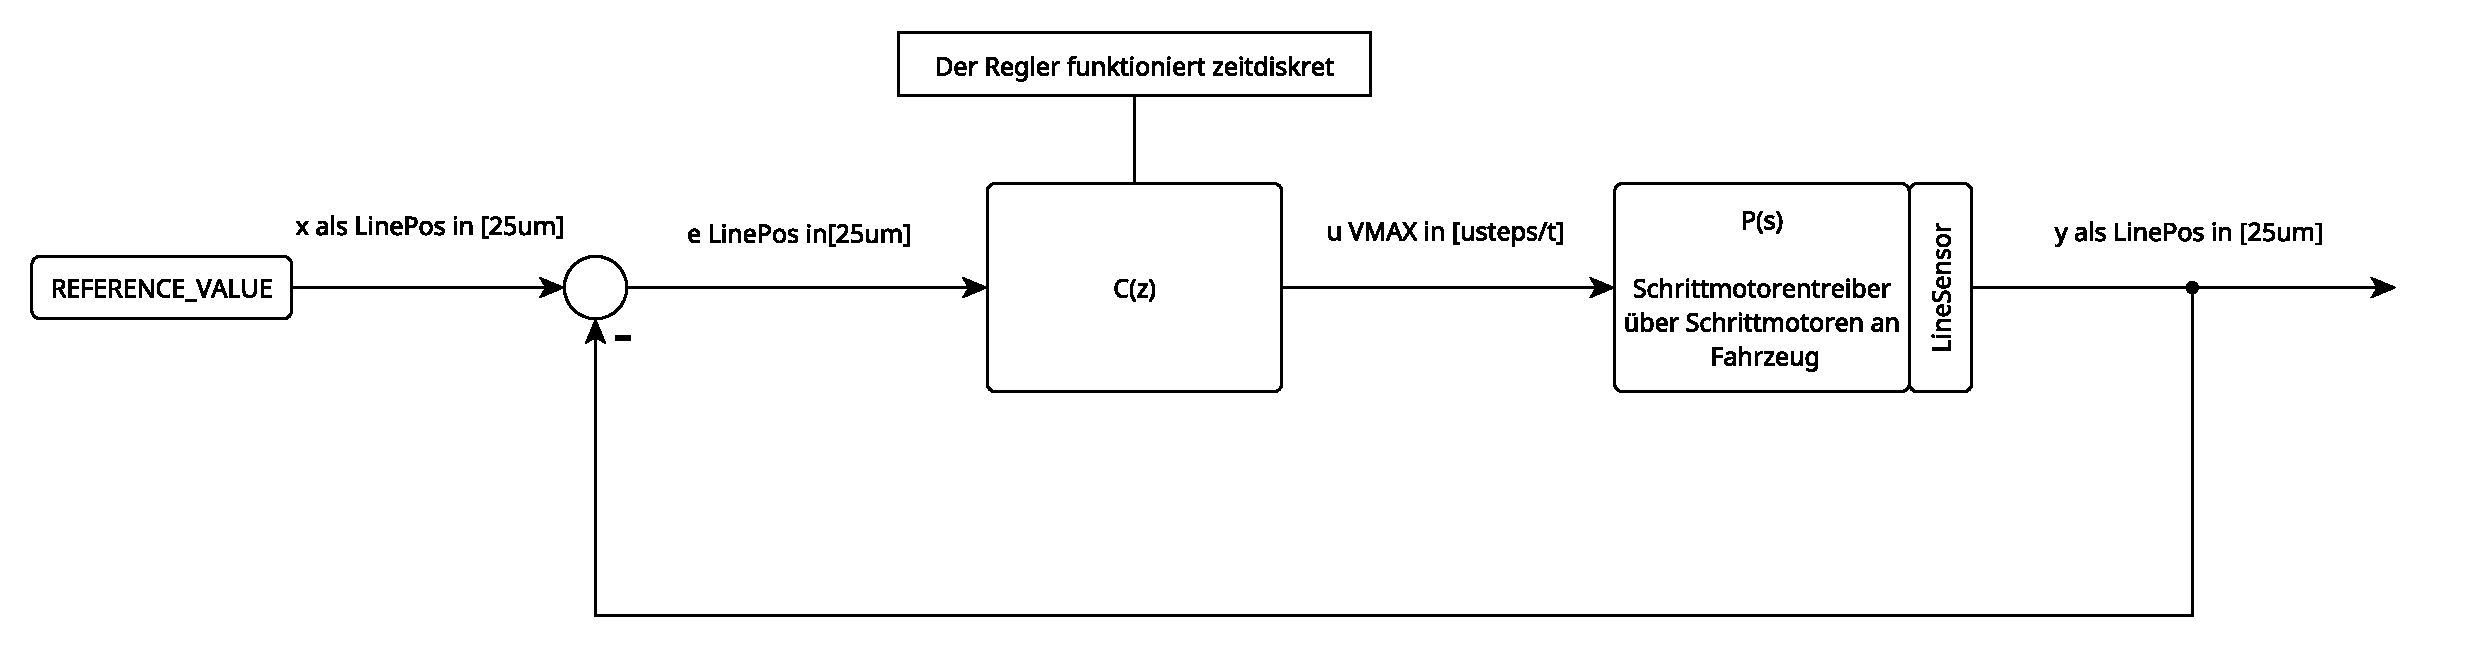
\includegraphics[width=1.0\linewidth]{../../Anhang_subfiles/Anhang_Elektronik/fig_Parametrierung_Linienfolgeregler/RegelProzess_Linienfolger.pdf}
    \caption{Reglerprozess des Linienfolgers}~\label{fig:Linienfolger_RegelProzess_ht}
\end{figure}

Der vereinfachte Regelkreis ist in
Abbildung~\ref{fig:Linienfolger_RegelProzess_ht} dargestellt. Die Grösse $x[k]$
bezeichnet, wie bereits erwähnt, die Referenzposition. Zusammen mit der
aktuellen Linienposition $y[k]$ wird die Regelabweichung $e[k]$ bestimmt. Die
Grössen in der Einheit der Linienposition ($x[k]$, $y[k]$ und $e[k]$) haben
aufgrund der Messauflösung der Zellen alle die Einheit $25 \mu m$. Der
dargestellte Block $C(z)$ repräsentiert den im MotionController implementierten
zeitdiskreten Regler. Seine Ausgangsgrösse $u[k]$ hat die Einheit $\frac{\mu
        \text{steps}}{t}$ und beschreibt die Motordrehzahl, die an den Prozess $P(s)$
weitergegeben wird. Die Ausgangsgrösse des Prozesses $P(s)$ wird wiederum vom
Linearsensor erfasst und durch die Grösse $y[k]$ dargestellt.

Jeder Motor wird bei Geradeausfahrt mit einer vorgegebenen Maximaldrehzahl
\texttt{V\_MAX\_USTEPS\_PER\_T} angesteuert. Zu dieser Geschwindigkeit wird bei
einem Motor die Regelgrösse $u[k]$ addiert, bei dem anderen subtrahiert.
Dadurch dreht sich das Fahrzeug bei einer Regelabweichung um den
Achsmittelpunkt.

In der Firmware des MotionControllers ist der ermittelte PD-Regler mittels
\textit{Tustin - Approximation} in den Zeitdiskreten bereich übertragen worden
und ist wie nachfolgend dargestellt als differenzengleichung implementiert:

\[
    u[k] = \beta \cdot e[k] - \beta \cdot e[k - 1] + \alpha \cdot u[k - 1]
\]

\subsubsection*{Steuerungsablauf bei Hindernissen}

Der Bewegungsablauf wird von einer Zustandsmaschine gesteuert, die im
BarrierHandler-Task implementiert ist. Nachfolgend wird lediglich der
Bewegungsablauf beschrieben. Genauere Details zu dieser Zustandsmaschine sind
im Anhang~\ref{apdx:HandlerBarrierStm} dokumentiert.

\begin{enumerate}
    \item Hindernisse, die sich näher als $500$ mm befinden, werden überwacht. Wird ein
          Hindernis in Abbremsreichweite erkannt, wird das Fahrzeug zunächst leicht
          verlangsamt, um die Samplingrate des Ultraschallsensors zu erhöhen.

    \item Sobald sich das Hindernis in einer Distanz befindet, die dem Bremsweg
          entspricht, wird das Fahrzeug abgebremst.

    \item Nachdem das Fahrzeug zum Stillstand gekommen ist, wird aus einer Messreihe von
          Distanzwerten erneut der Median berechnet und die Position ein letztes Mal
          korrigiert.

    \item Sobald sich der Greifer korrekt über dem Hindernis befindet, wird der
          GripController angewiesen, das Hindernis aufzunehmen.

    \item Ist das Hindernis gegriffen, dreht sich das Fahrzeug um $180^\circ$ und bewegt
          sich eine Fahrzeuglänge rückwärts.

    \item Der GripController wird angewiesen, das Hindernis abzusetzen.

    \item Nach Erhalt der Bestätigung des GripControllers bewegt sich das Fahrzeug ein
          kleines Stück zurück und dreht sich erneut um $180^\circ$.

    \item Das Hindernishandling ist abgeschlossen, und die Fahrt kann fortgesetzt werden.
          Der LineFollowerTask wird angewiesen, die Linienverfolgung fortzusetzen.
\end{enumerate}

Die Steuerung des Fahrzeugs, einschliesslich Drehungen und Positionsänderungen,
erfolgt ausschliesslich über die bereits erwähnten \texttt{DispatcherMessage}s,
die vom MessageDispatcher an die jeweiligen Tasks weitergeleitet werden.

Um diese \textit{manuellen} Bewegungen auszuführen, ist im LineFollowerTask
eine eigene Zustandsmaschine implementiert, die die Kommandos \texttt{Stop},
\texttt{Move} und \texttt{Turn} ausführen kann. Weitere Details zu diesem
Zustandsautomaten sind im Anhang~\ref{apdx:MovePositionModeStm} beschrieben.

\subsubsection*{Schrittmotoren und deren Ansteuerung}

Es werden die aus PREN1 evaluierten Schrittmotoren zusammen mit den
Motorentreibern \textit{ADI-Trinamic TMC5240} eingesetzt. Diese Motorentreiber
bieten eine einfache Schnittstelle zur präzisen Steuerung der Motoren. Für die
Linienfolgefunktion werden die Motoren im \textit{Velocity Mode} betrieben, bei
dem der Treiber eine vorgegebene Drehzahl automatisch einregelt.
Positionierungsaufgaben werden im \textit{Position Mode} ausgeführt, bei dem
dem internen Schrittzähler des Motorentreibers Sollpositionen vorgegeben
werden, die er dann selbstständig anfährt.

Ein Motor wird gestoppt, indem ihm im \textit{Velocity Mode} eine Soll-Drehzahl
von $0 \frac{\mu \text{steps}}{t}$ vorgegeben wird.

Die Motorentreiber sind über SPI mit dem MotionController verbunden. Über diese
Schnittstelle werden sämtliche Konfigurationen und Befehle an die
Motorentreiber übertragen.

% ABBILDUNG ADI TMC5240 EVAL BOARD PREN1

\end{document}
